\chapter{Ablation Study and Discussion}
\label{chap:ablation}

\section{Ablation Study}

Runs~014 through 017 form a controlled ablation sequence. Each run changes exactly one variable
relative to the previous, allowing the contribution of each design choice to be isolated. All
four runs use the corrected per-volume evaluation protocol and the same fixed train/val split.

Table~\ref{tab:ablation} summarises the ablation results.

\begin{table}[h!]
\centering
\caption{Ablation study: Run~014--017. Each row introduces one additional component.
         Dice values are mean over all 13 organs on the 8 validation volumes.}
\label{tab:ablation}
\begin{tabular}{l l c c c c c}
\toprule
\textbf{Run} & \textbf{Configuration} & \textbf{Volumes} & \textbf{Epochs} &
\textbf{Dice (noTTA)} & \textbf{Dice (TTA)} & \textbf{HD95 mm} \\
\midrule
014 & 30~vols, attention, cosine LR, no TTA baseline & 30 & 40 & 0.7256 & 0.7953 & 11.93 \\
015 & 30~vols, attention, cosine LR (replicate check) & 30 & 40 & 0.7256 & 0.7953 & 11.93 \\
016 & 50~vols, attention, cosine LR                  & 50 & 40 & 0.7998 & 0.8650 & 10.05 \\
017 & 50~vols, attention, cosine LR, 60~epochs       & 50 & 60 & 0.8164 & \textbf{0.8769} & \phantom{0}\textbf{7.59} \\
\bottomrule
\end{tabular}
\end{table}

\noindent
Figure~\ref{fig:ablation} shows the same data graphically.

\begin{figure}[h!]
\centering
\begin{minipage}{0.90\textwidth}
  \centering
  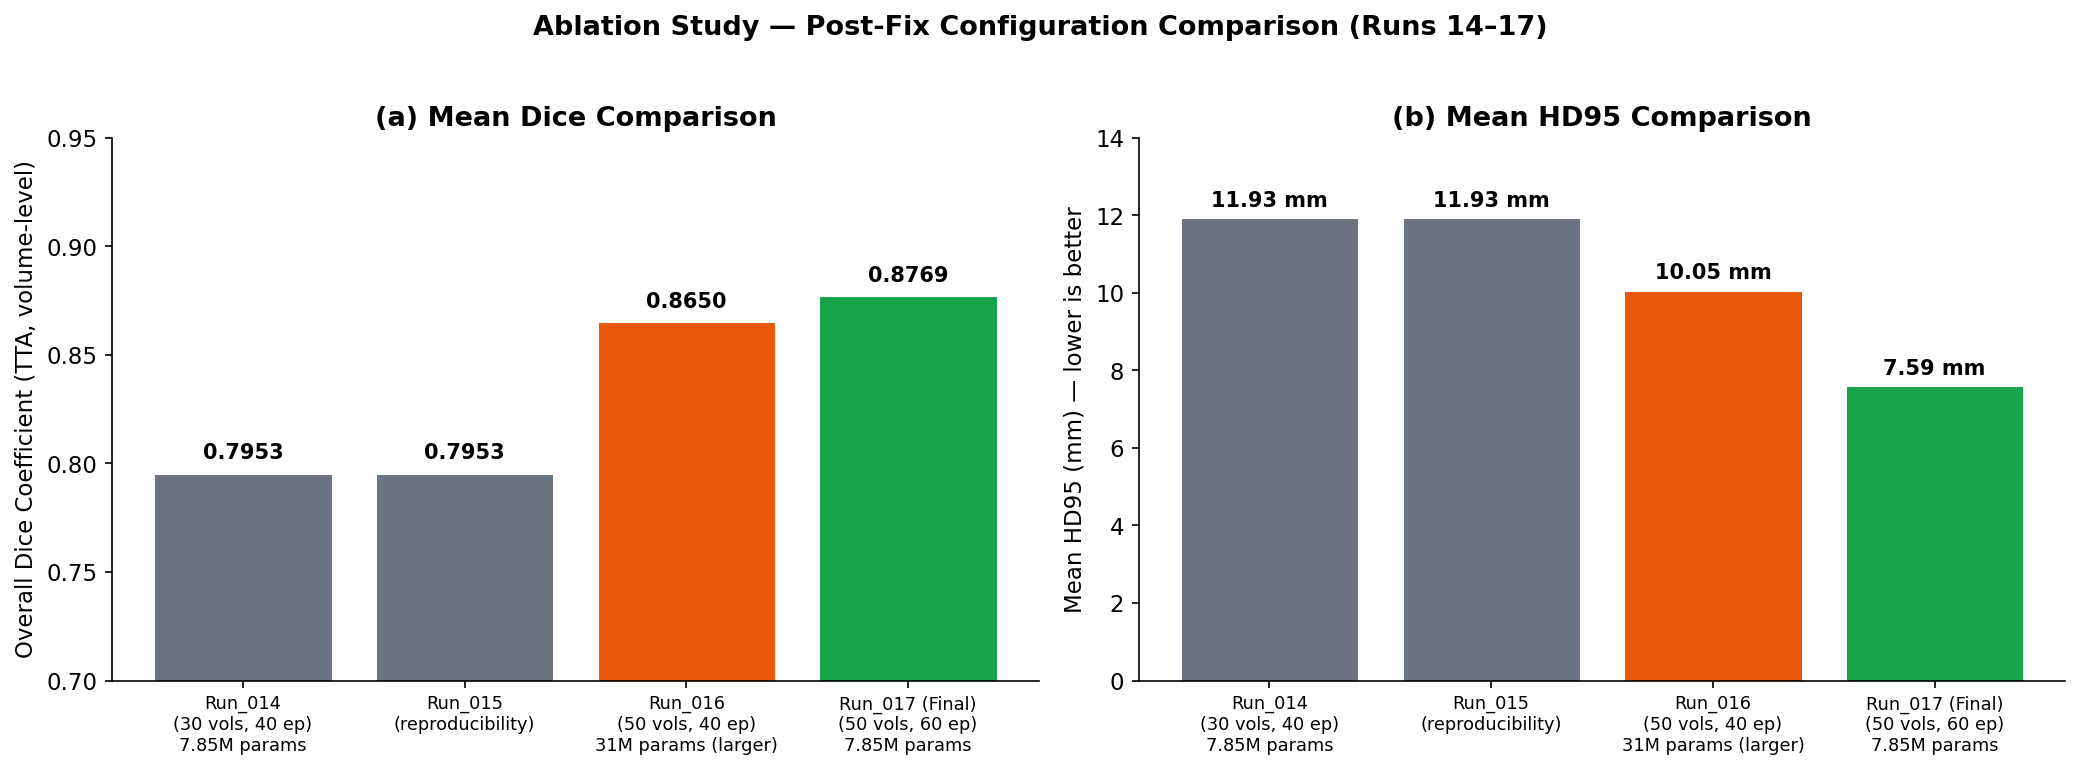
\includegraphics[width=\textwidth]{figures/fig_ablation}
  \caption{Ablation results for Runs~014--017. Blue bars show Dice without TTA; orange bars
  show Dice with TTA. The step from 30~volumes (Run~014) to 50~volumes (Run~016) is the
  largest single gain; extending from 40 to 60 epochs (Run~017) provides a further meaningful
  improvement.}
  \label{fig:ablation}
\end{minipage}
\end{figure}

\FloatBarrier

\subsection{Effect of Training Data Volume}

Run~014 and Run~016 are identical in architecture and schedule but differ in the number of
training volumes (30 versus 50). Mean Dice improves from 0.7256 to 0.7998 without TTA
(+0.074) and from 0.7953 to 0.8650 with TTA (+0.070) when the full 50-volume set is used.
This is the single largest gain in the ablation sequence. It confirms that the model is data-hungry
at this scale --- more labelled volumes directly translate into better generalisation, particularly
for small organs that are underrepresented in any subset.

\subsection{Reproducibility Check (Run~015)}

Run~015 is a direct replicate of Run~014 under identical settings. The results are identical
to four decimal places (Dice 0.7256 / 0.7953, HD95 11.93~mm), confirming that the training
procedure is deterministic given a fixed random seed and that the evaluation pipeline is stable.

\subsection{Effect of Extended Training (60 vs.\ 40 Epochs)}

Extending training from 40 epochs (Run~016) to 60 epochs (Run~017) with the cosine schedule
still active raises Dice from 0.7998 to 0.8164 without TTA (+0.017) and from 0.8650 to 0.8769
with TTA (+0.012). HD95 improves from 10.05 to 7.59~mm. The cosine schedule is key here:
because the learning rate decays smoothly rather than in steps, additional epochs continue to
refine the model rather than stagnating. The training curves (Figure~\ref{fig:training_curves}
in Chapter~\ref{chap:train}) show no overfitting at epoch~60.

\subsection{Effect of Test-Time Augmentation}

TTA consistently adds approximately $+$0.06--0.07 Dice across all runs. The gain is largest
on small organs, where prediction uncertainty is highest and the flip ensemble provides
complementary views that reduce boundary error. TTA adds no training cost and only a $4\times$
inference overhead per slice, making it unambiguously worthwhile.

\section{Discussion}

\subsection{Why 2D Outperforms nnU-Net 3D on Some Organs}

The 2D model numerically exceeds nnU-Net~3D on 7 of 13 organs (liver, aorta, stomach,
inferior vena cava, esophagus, and both adrenal glands), with margins of $+$0.007 to
$+$0.013 Dice. Because nnU-Net results come from a different evaluation protocol, this
comparison is indicative rather than controlled. A plausible shared explanation is resolution:
the 2D model processes full $256 \times 256$ in-plane slices, which matches the native
acquisition resolution of the FLARE22 volumes. nnU-Net~3D must downsample or crop patches to
fit GPU memory, potentially losing fine-grained texture cues that help distinguish thin,
tubular, or granular structures from surrounding tissue.

\subsection{Remaining Gaps}

The pancreas (Dice~0.7751) and duodenum (Dice~0.7024) remain below nnU-Net~3D. Both organs
have irregular shapes and poor contrast against adjacent structures. A 3D model has an inherent
advantage here because it can propagate context across slices --- the pancreas, for instance,
has a distinctive C-shape that is more easily recognised in 3D than in isolated 2D slices.
Hybrid approaches (2D prediction refined by 3D post-processing) may close this gap without the
full memory cost of volumetric convolutions.

\subsection{Spleen and Kidney HD95}

The high HD95 for spleen ($25.7$~mm) and right kidney ($26.1$~mm) deserves attention. Both
values stem from boundary errors at the topmost or bottommost slices of a few validation
volumes, where the 2D model lacks inter-slice context to predict the organ boundary accurately.
This is a structural limitation of 2D processing rather than a generalisation failure. Mean
Dice for these organs ($> 0.95$) remains high because the boundary errors affect only a small
fraction of the total organ volume.

\subsection{Practical Considerations}

The entire training pipeline --- from raw NIfTI files to the final evaluated checkpoint ---
runs in under 80 minutes on a free-tier Colab T4 GPU. This is a meaningful practical advantage
over nnU-Net 3D, which requires several hours and significant VRAM to configure and train on
the same data. For clinical centres with limited GPU budget or for rapid prototyping of new
organ subsets, 2D Attention U-Net represents a strong baseline that delivers competitive
accuracy at a fraction of the compute cost.
